\documentclass[a4paper,titlepage,12pt]{article}
\usepackage[utf8]{inputenc} %Make sure all UTF8 characters work in the document
\usepackage{graphicx}
\usepackage{titling}
\usepackage{tabularx}
\usepackage{longtable}
\usepackage[yyyymmdd]{datetime}
\usepackage[figurename=Figur]{caption}
\usepackage{booktabs}
\usepackage[parfill]{parskip}

%Set page size
\usepackage{geometry}
\geometry{margin=3cm}

\renewcommand{\dateseparator}{-}
\renewcommand{\contentsname}{Innehållsförteckning}
\renewcommand{\tablename}{Tabell}


\usepackage{listings}
\usepackage{color}

\usepackage[colorinlistoftodos,prependcaption,textsize=tiny]{todonotes}

\definecolor{dkgreen}{rgb}{0,0.6,0}
\definecolor{gray}{rgb}{0.5,0.5,0.5}
\definecolor{mauve}{rgb}{0.58,0,0.82}

\lstset{frame=tb,
  language=Python,
  aboveskip=3mm,
  belowskip=3mm,
  showstringspaces=false,
  columns=flexible,
  basicstyle={\small\ttfamily},
  numbers=none,
  numberstyle=\tiny\color{gray},
  keywordstyle=\color{blue},
  commentstyle=\color{dkgreen},
  stringstyle=\color{mauve},
  breaklines=true,
  breakatwhitespace=true,
  tabsize=3
}

%%%%%%%%%%%%%%%%%%%%%%%%%%%%%%%
% Header and footer
%%%%%%%%%%%%%%%%%%%%%%%%%%%%%%%
\usepackage{fancyhdr}
\pagestyle{fancy}

\lhead{
\includegraphics[width=0.15\linewidth]{../images/logo_full.png}}
\chead{Teknisk dokumentation för sexbent robot}
\rhead{\today}
\setlength\headheight{26pt} 

\lfoot{TSEA29 -- KMM \\ LIPS Teknisk Dokumentation}
\rfoot{Grupp 9 \\ LiTHe Hex}

\newcommand{\itc}{I\textsuperscript{2}C}

\pretitle{%
	\begin{center}
		\LARGE
		
\includegraphics[width=6cm]{../images/logo_full.png}\\[\bigskipamount]
}

\posttitle{\end{center}}

\begin{document}
\listoftodos
	\title{\LARGE
		\textbf{Teknisk dokumentation för sexbent robot} \\
		\vspace*{0.5\baselineskip}
		\large
		Redaktör Frans Skarman \\
		Grupp 9 \\
		\small
		\vspace*{0.5\baselineskip}
		Version 0.1}

	\date{\today}

	\maketitle
	
	\newpage
	
	\begin{center}

		%%%%%%%%%%%%%%%%%%%%%%%%%%%%%%%%%%%%%%%%%%%%%%%%%%%%%%%%%%%%%%%%%%%%%%%%%%%%%%%%%
		%						Medlemmar
		%%%%%%%%%%%%%%%%%%%%%%%%%%%%%%%%%%%%%%%%%%%%%%%%%%%%%%%%%%%%%%%%%%%%%%%%%%%%%%%%%

		\section*{Projektidentitet}
		Grupp 9, Ht 2016, LiTHe Hex

		Linköpings Tekniska Högskola, ISY

		\renewcommand*{\arraystretch}{1.4}
		\begin{longtable}[c]{ l l l }
			\textbf{Namn} & \textbf{Ansvar} & \textbf{E-post} \\ \midrule
			Emil Segerbäck & & emise935@student.liu.se \\ \midrule
			Frans Skarman & Dokumentansvarig & frask812@student.liu.se \\ \midrule
			Hannes Tuhkala & & hantu447@student.liu.se \\ \midrule
			Malcolm Vigren & Projektledare & malvi108@student.liu.se \\ \midrule
			Noak Ringman &  & noari093@student.liu.se \\ \midrule
			Olav Övrebö &  & olaov121@student.liu.se \\ \midrule
			Robin Sliwa &  & robsl733@student.liu.se \\
		\end{longtable}

		\centering
		\textbf{Kursansvarig}: Tomas Svensson Rum 3B:528 013--28 13 68 tomas.svensson@liu.se

		\newpage
		\tableofcontents
		\newpage


		%%%%%%%%%%%%%%%%%%%%%%%%%%%%%%%%%%%%%%%%%%%%%%%%%%%%%%%%%%%%%%%%%%%%%%%%%%%%%%%%%
		%						Historik
		%%%%%%%%%%%%%%%%%%%%%%%%%%%%%%%%%%%%%%%%%%%%%%%%%%%%%%%%%%%%%%%%%%%%%%%%%%%%%%%%%

		\section*{Dokumenthistorik}
		\renewcommand*{\arraystretch}{1.4}
        \begin{longtable}[c]{ l l >{\raggedright}p{5cm} >{\raggedright}p{3cm} l }
			\textbf{Version} & \textbf{Datum} & \textbf{Utförda förändringar} 
			& \textbf{Utförda av} & \textbf{Granskad} \\ \midrule
			
			0.1 & 2016--10--20 & Första utkastet & Projektgruppen &
            Projektgruppen \\
            
		\end{longtable}
	\end{center}

	%%%%%%%%%%%%%%%%%%%%%%%%%%%%%%%%%%%%%%%%%%%%%%%%%%%%%%%%%%%%%%%%%%%%%%%%%%%%%%%%%
	%						Inledning
	%%%%%%%%%%%%%%%%%%%%%%%%%%%%%%%%%%%%%%%%%%%%%%%%%%%%%%%%%%%%%%%%%%%%%%%%%%%%%%%%%

	\newpage

	\raggedright

	\section{Inledning}
	Detta dokument går i detalj in på konstruktionen och mjukvaran för en 
	sexbent robot, med autonom och manuell styrning. Först presenteras en 
	översiktlig beskrivning av robotens styrande processorer ("enheter", vilka kopplas till ett färdigt 
	PhantomX AX Metal Hexapod Mark III chassi från TrossenRobotics). Dessa (central-, 
	motorik- och sensorenhet), kommunikation mellan dessa, samt användargränssnitt specificeras 
	sedan i större noggrannhet under egna avdelningar.

	%%%%%%%%%%%%%%%%%%%%%%%%%%%%%%%%%%%%%%%%%%%%%%%%%%%%%%%%%%%%%%%%%%%%%%%%%%%%%%%%%
	%						Översikt
	%%%%%%%%%%%%%%%%%%%%%%%%%%%%%%%%%%%%%%%%%%%%%%%%%%%%%%%%%%%%%%%%%%%%%%%%%%%%%%%%%

	\section{Systemöversikt}
	Systemet innehåller tre enheter. En centralenhet implementerad på en Raspberry Pi 3 
	agerar som master för de andra två (slav-)processorerna. Denna står för all kommunikation 
	med omgivningen genom en webserver som datorer kan koppla upp sig mot för att styra roboten 
	eller få tillgång till debugdata. I autonomt läge är det även denna enhet som utifrån 
	insamlad data fattar alla styrande beslut utifrån vilka de andra enheterna
  verkar. Vid manuell styrning vidarebefordras endast data från styrdatorn.

	De två andra enheterna (slavarna till centralenheten) utgörs av AVR-processorer och styr 
	mer generella uppgifter. Den ena, motorikenheten, översätter generella indikationer om 
	förflyttning från centralenheten till faktiska kommandon för robotens servon, och skickar 
	vidare dessa. Den kan även förse centralenheten med bland annat debugdata om så efterfrågas.
	
	Den andra AVR-processorn utgör en sensorenhet, vilken styr och läser robotens sensorsvit. 
	Den svarar även för att översätta råa sensordata till mer konkreta former (som vinklar och 
	avstånd), samt att brusreducera dessa efter behov. Figur \ref{fig:overview} ger en översiktsbild av
	systemet.
	\begin{figure}[h!]
		\centering
		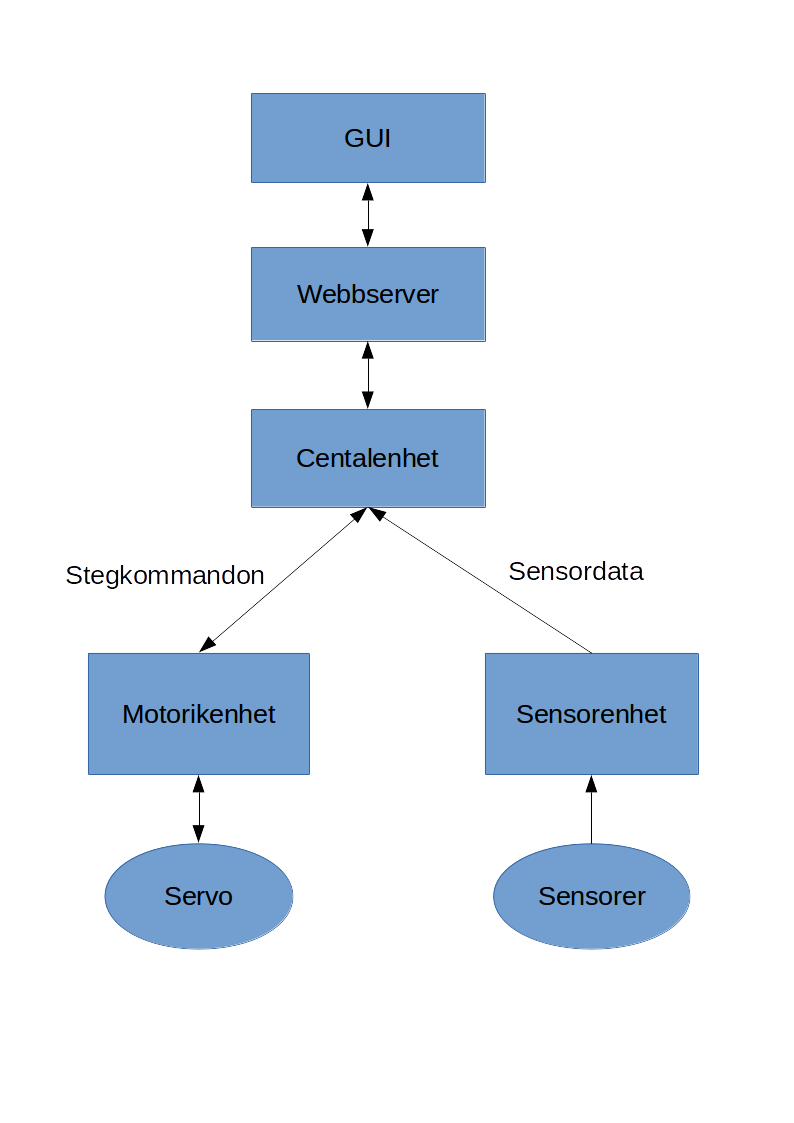
\includegraphics[width=0.5\linewidth]{../images/overview.png}
		\caption{Översikt av systemet\label{fig:overview}}
	\end{figure}

	\newpage

	\subsection{Kommunikation mellan enheterna}
	Kommunikation mellan centralenheten och de två AVR-processorerna sker
	med SPI. Sensor- och motorikenhetens SPI-portar kopplas till centralenhetens
	SPI-port med varsin chip select. Detta illustreras i figur \ref{fig:central_circuit}.
	All kommunikation inleds med att 
	centralenheten skickar ett kommando eller en databegäran till slavenheterna.
	Slavenheterna utför sedan kommandot eller svarar med den begärda datan.

	\begin{figure}[htpb]
		\centering
		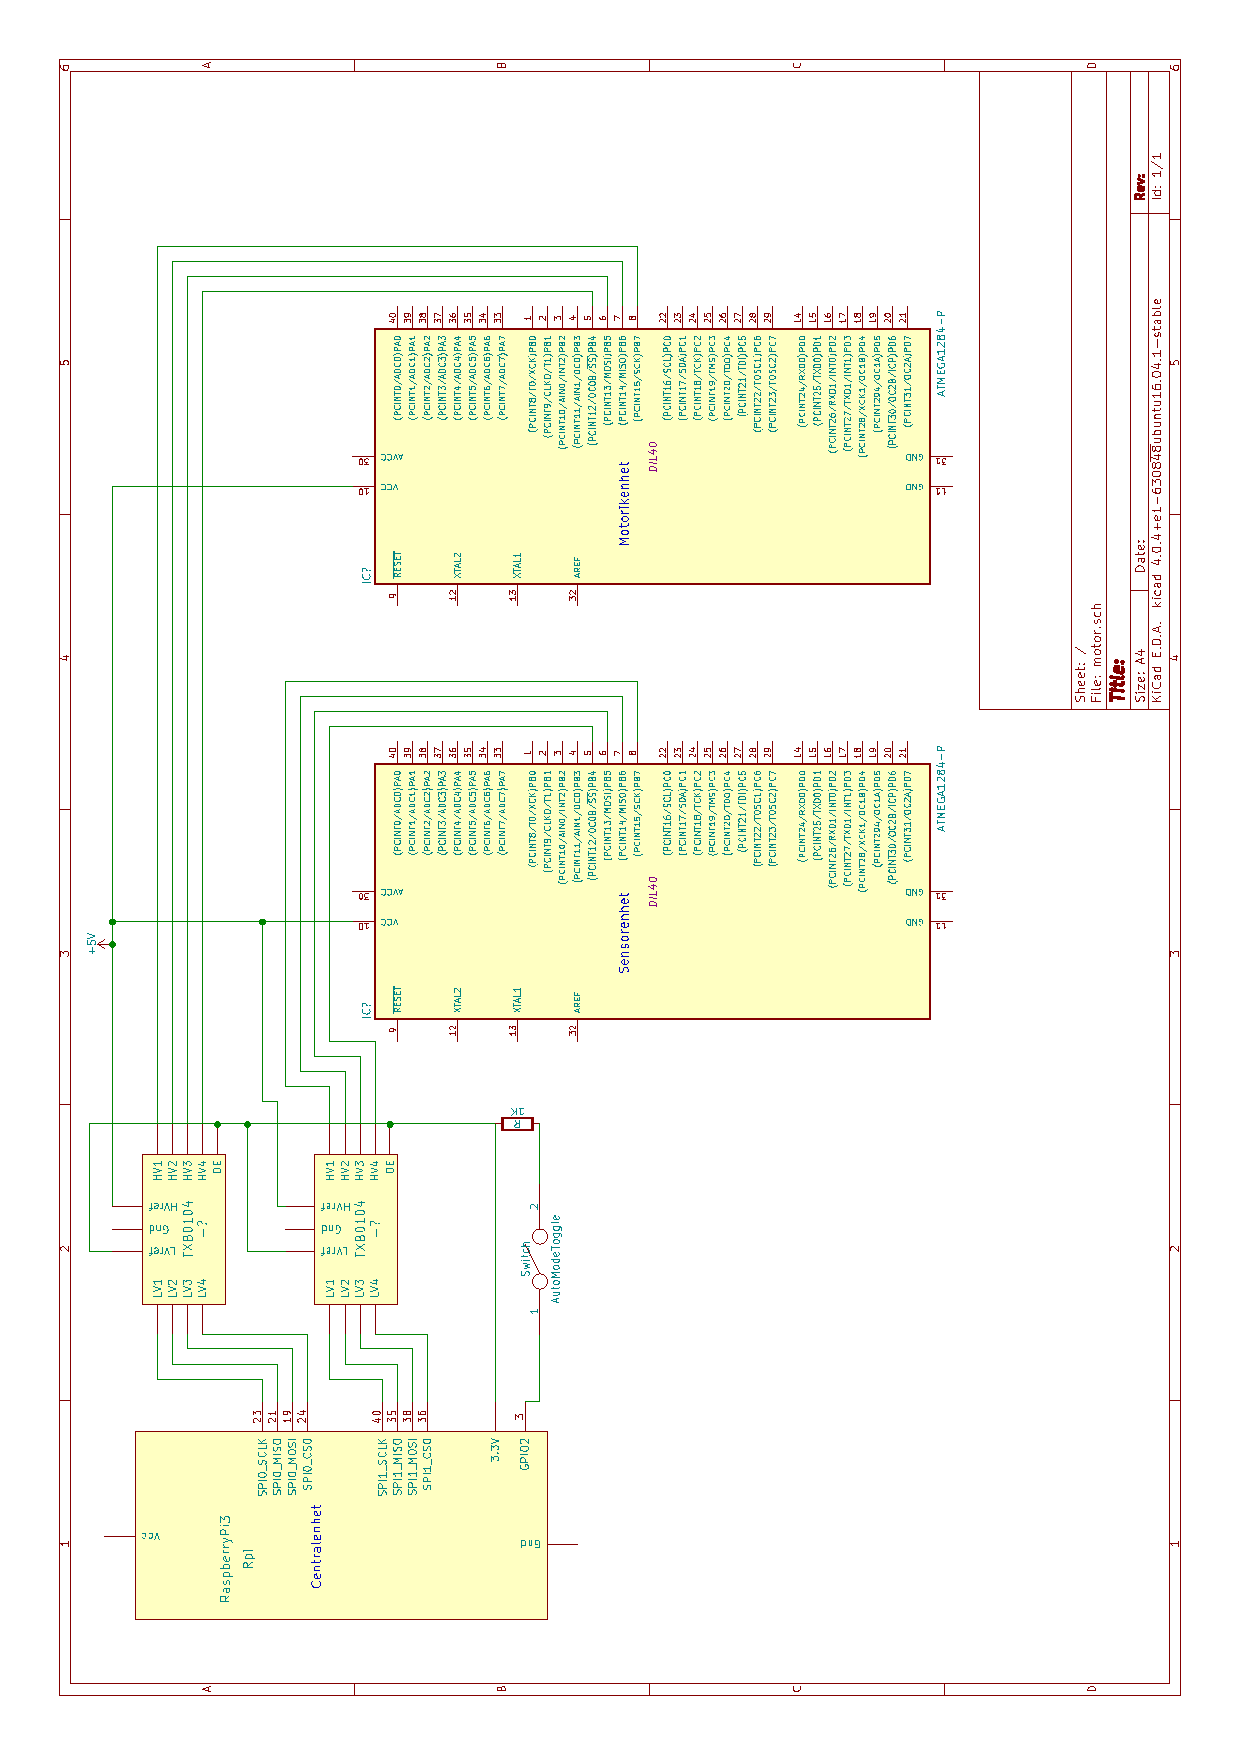
\includegraphics[width=1.0\linewidth]{charts/central/centralenhet.pdf}
		\caption{Kopplingsschema för centralenheten}
		\label{fig:central_circuit}
	\end{figure}




	\subsubsection{Kommunikationsprotokoll}
	\label{ssub:Kommunikationsprotokoll}
	Kommunikationen mellan centralenheten, motorikenheten och sensorenheten sker 
	med protokollet som beskrivs i figur \ref{fig:kommunikation1}.

	\newpage
	\begin{figure}[h!]
		\centering
		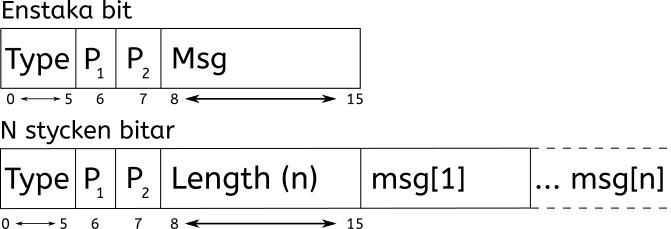
\includegraphics[width=0.5\linewidth]{images/communication_protocol1.png}
		\caption{Översiktlig vy av kommunikationsprotokolllet}
		\label{fig:kommunikation1}
	\end{figure}

	De första 6 bitarna av varje meddelande säger vilken typ av meddelande det är som
	skickas, dessa beskrivs i tabell 
	\ref{table:messages}. Den första biten i typparametern är 0 om meddelandets
	innehåll är en enstaka byte och 1 om meddelandet har dynamisk längd. Om längden
	är dynamisk är första byten i meddelandet längden av resten av meddelandet.

	De två sista bitarna i första byten är paritetsbitar. Bit 7 är en  paritetsbit
	för meddelandets innehåll medan bit 8 är paritetsbit för de 7 tidigare bitarna.

	Om någon av paritetsbitarna är fel så kommer enheten som tog emot meddelandet att svara
	med ett speciellt meddelande för att indikera sändningsfel. Annars kommer den 
	att svara med ett "acknowledgemeddelande".

    \newpage
	\begin{longtable}[c]{ l l l }
		\textbf{Syfte} & \textbf{ID} & \textbf{Data} \\ \midrule
		\textbf{Generella} \\ \midrule
		Send fail & 1F & -- \\ \midrule
		Acknowledge & 0F & -- \\ \midrule
		Datarequest & 02 & data \\ \midrule
		\\
		\textbf{Centralenhet $ \to $ motorikenhet}\\ \midrule
		Sätt hindergång & 03 & på/av \\ \midrule
		Sätt servohastighet & 20 & 8 LSD, 8 MSD \\ \midrule
		Gåkommando &  21 & len, x- och y-hastighet, svänghastighet,
        autonom-läge \\ \midrule
		Return to neutral & 05 & -- \\ \midrule
		\\
		\textbf{Centralenhet $ \gets $ motorikenhet}\\ \midrule
		Servostatus & 22 & len, ... data ... \\ \midrule
		Debugsträng & 23 & len, "debugsträng i utf-8" \\ \midrule
		Upptagen med rotation? & 03 & ja: 0x01, nej: 0x00 \\ \midrule
		\\
		\textbf{Centralenhet $\to$ sensorenhet} \\ \midrule
		Återställ orientering & 03 & -- \\ \midrule
		\\
		\textbf{Centralenhet $ \gets $ sensorenhet}\\ \midrule
		Behandlad sensordata & 24 & len,ir-ner, ir-fv, ir-bv, ir-fh, ir-bh,
        lidar-lsd, lidar-msb \\ \midrule
		Korridordata		 & 25 & len, avst. fram, vänster, höger, ned, vinkel \\

		\caption{Meddelandespecifikation \label{table:messages}}
	\end{longtable}

	\newpage
	Algoritmen för läsning av data i centralenheten beskrivs av följande pseudokod.


	%Pseudocode for reading replies
	\begin{lstlisting}
	def read_reply():
		set_chip_select()

		set byte = read_byte_when_available()

		set type = byte[0..5]
		if(byte[0] == 0)
			set length = 1
		else
			set length = read_byte_when_available()
		
		result = []
		for i = 0..length:
			result.append(read_byte_when_available())

		if check_parity_bits() == good
			return (Ok, type, result)
		else
			return (Fail, 0, [])
	\end{lstlisting}

	Algoritmen för att skicka data till andra enheter beskrivs i följande pseudokod.

	\begin{lstlisting}
	def write_to_module(msg):
		set_chip_select()

		write_to_spi(msg)

		set reply = read_reply()

		if reply.status == OK and reply.type == ACK:
			return
		else:
			write_to_module(msg)
	\end{lstlisting}


	\newpage
	Algoritmen för att skicka och ta emot data på motorik- och sensorenheten beskrivs
	i följande pseudokod

	\begin{lstlisting}
		#Init
		set activate_interrupts_for_spi()
		set received_msgs = new Queue()

		set current_msg = []

		#Event handler for spi messages
		def on_spi_recv(byte):
			current_msg += byte

			if msg_is_complete:
				set success = check_parity()
				if success == OK:
					send_ack()
				
				if message requires reply:
					send_reply()
				else:
					received_msgs.push(current_msg)
	\end{lstlisting}

	
	\section{Komponentbudget}

    Tabell \ref{table:components} visar komponenter som ingår i
    roboten, utöver chassiet, lödplattor och andra diverse
    mindre komponenter.

	\begin{longtable}[c]{l l}
		\textbf{Komponent} & \textbf{Antal} \\ \midrule
		Raspberry Pi 3 & 1 \\
		ATmega1284 & 2 \\
		GP2D120 & 1 \\
		GP2Y0A02YK & 4 \\
		MLX90609 & 1 \\
		LIDAR Lite, V2 eller V3 & 1 \\
	    74LS240 & 8 \\
        Extern 16 MHz-klocka EXO-3 & 1 \\
        TXB0104 & 2 \\
        \caption{De komponenter som beräknas att gå åt \label{table:components}}
	\end{longtable}
	
    \newpage
	\section{Centralenheten}
	Centralenheten har tre ansvarsområden: navigation/beslutsfattning, hinderdetektion samt
	kommunikation med omvärlden.

	\subsection{Navigation och beslutsfattning}
	Centralenheten sköter all beslutsfattning om hur roboten ska röra sig
	genom labyrinten. Den tar emot data från sensorenheten och GUI:t och
	skickar kommandon till motorikenheten.
  
	\subsubsection{Autonomt läge}
	I det autonoma läget frågar centralenheten om data från sensorenheten
    varje gång det ska fattas ett beslut. Detta gör att centralenheten själv
    bestämmer när den ska ha ny data för att den inte ska bli avbruten eller missa
    data för att den är mitt i utförandet av en annan funktion. Utifrån denna data
    fattar centralenheten beslut om hexapodens färdriktning.

    I beslutsfattning ingår bland annat korridorreglering, svänga in i korridorer, detektera
    och undvika återvändsgränder och gå över hinder när det har upptäckts.

    Korridorregleringen sker med hjälp av de fyra IR-sensorerna som sitter på
    sidorna av roboten. En vinkel räknas ut med med datan från dessa som säger
    hur roboten är vinklad i en korridor. Regleringen sker samtidigt som när
    roboten går framåt för att få jämnare gång i korridoren. Detta uppnås genom
    att en offset från mitten av korridoren beräknas och används när roboten ska
    vrida sig tillbaka till mitten. Ju närmare mitten den är desto mindre kommer
    den att vrida sig mot mitten.

    \todo{Lägg till pseudokod för korridorreglering}%
    \begin{lstlisting}
    def regulate(sensor_data, decision_packet):
    \end{lstlisting}

    Förutom de fyra IR-sensorerna på sidorna används även LIDAR och en femte
    IR-sensor när beslut ska fattas. LIDAR-sensorn som är riktad framåt används
    för att undvika ingång i återvändsgränder framåt. När ett beslut om korridor
    eller återvändsgränd fattas används sidosensorerna för att detektera och
    bekräfta det som detekterats. Inget beslut fattas innan båda sidosensorerna
    har detekterat samma sak så att risken för felbeslut minskar. Den femte
    IR-sensorn är riktad nedåt för att detektera hinder i labyrinten.

    När ett beslut om vändning har tagits väntar koden tills att en hel vändning
    har skett. Detta görs genom att vänta tills roboten står rakt framåt m.h.a.
    den uträknade vinkeln men även genom att vänta tills motorikenheten svarar
    att en hel vändning har gjorts klart. När en hel vändning har skett går
    roboten framåt tills den har kommit in i den nya korridoren innan den börjar
    fatta beslut med sensordatan den får in. Detta för att ignorera korridoren
    som roboten kom från. 
    
    \begin{lstlisting}
    def get_decision(sesor_data, decision_packet):
        corridors_and_dead_angles = get_corridors_and_dead_angles(sensor_data)

        for value in corridors_and_dead_ends:
            if 3 corridors detected:
                decision = TURN_LEFT
            
            elif 2 corridors detected:
                if distance forward is greater than DEAD_END_DISTANCE:
                    decision = GO_FORWARD
                else:
                    if left corridor detected:
                        decision = TURN_LEFT
                    else:
                        decision = TURN_RIGHT
            
            elif 1 corridor detected:
                if distance forward smaller than one tile 
                   and greater than LIDAR_STOP_DISTANCE:
                   decision = GO_FORWARD
                elif left corridor detected:
                    decision = TURN_LEFT
                elif right corridor detected:
                    decision = TURN_RIGHT
                else:
                    decision = GO_FORWARD

            elif 0 corridors detected:
                if distance forward is greater than LIDAR_STOP_DISTANCE:
                    decision = GO_FORWARD
                else:
                    decision = TURN_LEFT
    
    if previous decision is TURN_LEFT or TURN_RIGHT:
        # A complete turn has been made
        if absolute value of the average angle is less than 10 degrees and
        turn has completed:
            decision = GO_FORWARD
            previous_decision = COMPLETE_TURN

    elif previous decision is COMPLETE_TURN:
        decision = GO_FORWARD
        previous_decision = COMPLETE_TURN
        
        # if the robot has entered the new corridor
        if robot is inside a corridor:
            prev ious_decision = GO_FORWARD
        
    \end{lstlisting}
    
    \subsubsection{Manuell navigation}
    För den manuella navigationen används RabbitMQ mellan webbservern
    och centralenheten. Det kommer in ett nytt meddelande med data för varje
    knapptryck/händelse som sker på GUI:t som centralenheten tolkar och överför
    till motorikenheten. 

	\subsection{Kommunikation}
	Centralenheten kommunicerar med en dator över WiFi. Datorns webbläsare 
	ansluter till centralenhetens webbserver, då kan man
	via webbgränssnittet styra roboten samt läsa av robotens loggar. 
		
	\subsubsection{Kommunikation med webbserver}
	Centralenheten skickar och hämtar kontinuerligt meddelanden ifrån RabbitMQ servern och är i JSON-format. Centralenheten skickar den data som gui:t
	behöver till RabbitMQ servern och webbservern läser sedan in den data som finns där.
	Den data som skickas mellan centralenheten till webbservern kan ses i
	tabell \ref{table:guimessagesfromcentral} och den data som skickas från webbservern till centralenheten kan ses i tabell \ref{table:guimessagestocentral} vid sektion \ref{gui:kommunikation}.

	%%%%%%%%%%%%%%%%%%%%%%%%%%%%%%%%%%%% %%%%%%%%%%%%%%%%%%%%%%%%%%%%%%%%%%%%%%%%%%%%%
	%						Motorikenheten
	%%%%%%%%%%%%%%%%%%%%%%%%%%%%%%%%%%%%%%%%%%%%%%%%%%%%%%%%%%%%%%%%%%%%%%%%%%%%%%%%%
    \newpage
	\section{Motorikenheten}
	Motorikenheten översätter kommandon från centralenheten till servokommandon. Den tar emot 
	instruktioner från centralenheten som anger steglängd, fart, rotation och riktning för 
	förflyttnnig. Motorikenheten behandlar detta, räknar ut en lämplig gångstil och 
	signalerar nödvändiga vinklar till de sex benen. Vissa delmoment i förflyttningen 
	görs hårdkodade. Ett kretschema för motorikenheten finns i figur \ref{fig:motorik}

	För att kunna kommunicera med servona i 1 MBAUD klockas motorikenheten med en 16 MHz 
	EXO3 klocka.

	\begin{figure}[htpb]
		\centering
		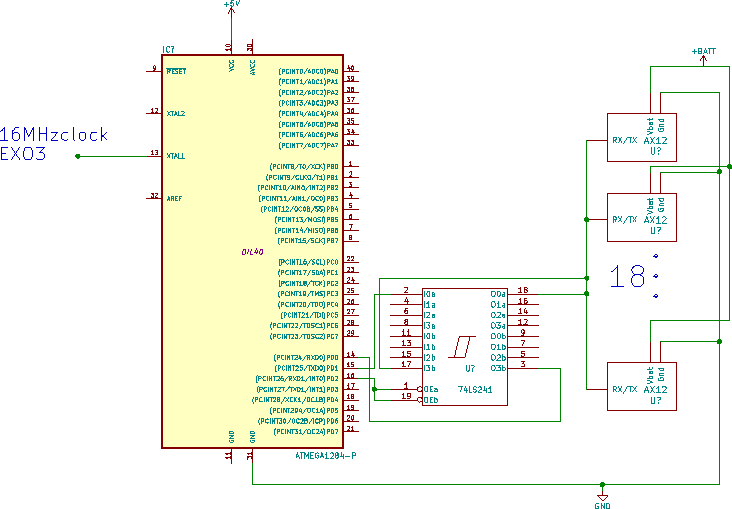
\includegraphics[width=0.6\linewidth]{charts/motor/motorik.pdf}
		\caption{Kretsschema för motorikenheten}
		\label{fig:motorik}
	\end{figure}
	
		\subsection{Planläggning}
	Första steget i motorikenheten för en anpassad gångstil är att utifrån efterfrågad
	förflyttning avgöra en önskad slutposition för respektive ben, som för roboten närmre 
	ett läge indikerat av centralenheten. Utifrån hastighet skalas förflyttningsvektorerna 
	från nuvarande läge för varje ben ner. Benen flyttas i grupper av tre med ett ben på 
	ena sidan och två på andra (uppdelat på ett mittenben, respektive ett framben och ett 
	bakben). När en uppsättning ben förflyttas, skiftas de markfästa benen vid behov för 
	att flytta själva kroppen, även denna utifrån en förflyttningsvektor (som med benen). 
	Lyft och nedsättning av ben hårdkodas, sådan att alla tre ben som skall flyttas i ett 
	set höjs och sänks först när de satts i önskad position, sådan att benens position 
	och förflyttning för vanlig gång kan beräknas i planet, snarare än i rummet, med 
	avseende på beslutsfattning. Endast vid den inverterade kinematiken krävs då 
	tredimensionell planering av benens rörelser. Detta beteende finns även illustrerat i 
	figur \ref{fig:walkflow0}. 
	
	För manuell styrning ska hastighet även kunna anpassas genom justering av servonas
	hastighetsinställning.

	\begin{figure}[h]
		\centering
		\includegraphics[width=0.5\linewidth]{images/gangstil_flowchart.png}
		\caption{Flödesschema för normal gångstil hos roboten \label{fig:walkflow0}}
	\end{figure}

	\subsection{Hindergång}
	För hindergång kan roboten treva med benen, och anpassa sig efter höjdskillnaden genom
	läsning av benens mötta motstånd. Benen sänks till det att de möter motstånd, dels
	vid uppstigning på hindret, men också vid gång på hindret (för att upptäcka när hindret 
	tar slut). Inför uppgång på hinder höjs även benen extra, för att tillåta kliven att nå 
	upp på hindret.

	Därtill gäller att benen flyttas marginellt (någon centimeter) vid uppkliv på eller 
	nedkliv från hinder. Detta för att undvika att fötterna hamnar instabilt på kanten till 
	hindret, samtidigt som roboten tycker sig stå stabilt. Detta underlättar även för att vid nedstig stödja benen 
	längre fram, för att undvika att falla framåt. En översikt över detta kan fås i figur \ref{fig:walkflow1}.

	\begin{figure}[h!]
		\centering
		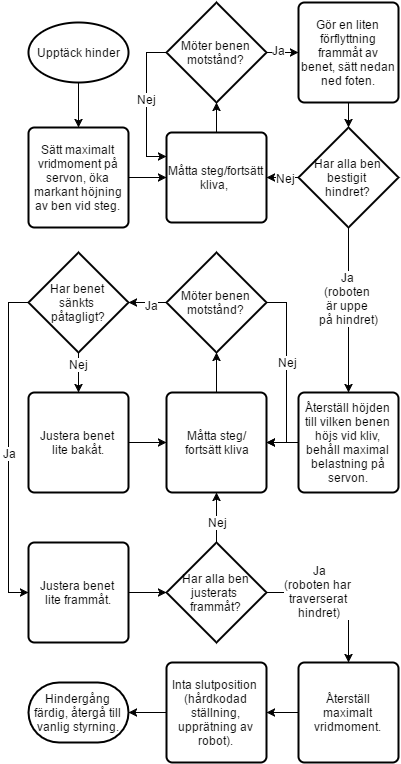
\includegraphics[width=0.5\linewidth]{images/hindergang_flowchart.png}
		\caption{Flödesschema för hindergångsprocedur hos roboten \label{fig:walkflow1}}
	\end{figure}

	\subsection{Inverterad kinematik}
	\label{sub:inverterad-kinematik}
	Då planläggningsdelen av motorikenheten beslutat om var ett ben skall flyttas beräknas 
	lämpliga vinklar för benets alla servon genom inverterad kinematik. Utifrån kända 
	längder på benen och positioner där man vill att fötterna ska placeras används 
	trigonometri för att avgöra slutgiltiga servovinklar.
	
	% TODO: Fix image by making it bigger and adding z, x, y..
	% or remake it
	Inverterad kinematik är ett 3D-problem men vi har delat upp det i två stycken 2D-problem istället. Z-axeln går rakt upp, x-axeln går jämt med roboten och y axeln går rakt ut med lederna. Det första 2D-problemet beräknar vinkeln mellan roboten och den innersta leden $\gamma$ och det andra 2D-problemet beräknar vinkeln $\alpha$ mellan första och andra leden samt vinkeln $\beta$ mellan andra och tredje leden. Se figur \ref{fig:ik}.
	
	% Add formulas for the different angles?
	
	\begin{figure}[h!]
		\centering
		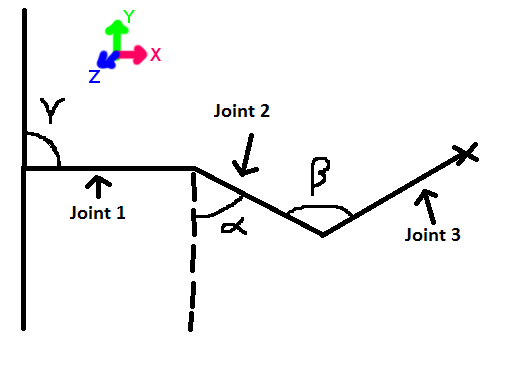
\includegraphics[width=0.5\linewidth]{images/ik.png}
		\caption{3D-problemet för IK med ett ben
		\label{fig:ik}}
	\end{figure}

	\subsection{Kommunikation med servon}
	Servona styrs via en UART-länk, med hjälp av addresserade datapaket. Vid behov, 
	som vid justering av hastighet, ändras inställningarna i servona själva, allt 
	utifrån metoden beskriven i databladet för AX-12-servon.
	
    

	%%%%%%%%%%%%%%%%%%%%%%%%%%%%%%%%%%%%%%%%%%%%%%%%%%%%%%%%%%%%%%%%%%%%%%%%%%%%%%%%%
	%						Sensorenheten
	%%%%%%%%%%%%%%%%%%%%%%%%%%%%%%%%%%%%%%%%%%%%%%%%%%%%%%%%%%%%%%%%%%%%%%%%%%%%%%%%%
	\section{Sensorenheten}
	Sensorenheten är den enhet som ger roboten sinnen för omvärlden, så att den
	kan navigera autonomt genom labyrinten. Sensorenheten är för
	centralenheten ett abstrakt gränssnitt till sensorerna. Centralenheten
	behöver alltså inte veta exakt vilka sensorer som används, utan istället
	läser av data som "avstånd till vägg", eller "vridning relativt väggarna".

	\subsection{Styrenhet i sensorenheten}
	Styrenheten för sensorenheten består av AVR-processorn ATmega1284, som läser av och 
	behandlar informationen från robotens sensorer. Styrenheten sköter även
	kommunikationen med centralenheten -- den tar emot förfrågningar om data och
	skickar behandlad data på begäran.

	Styrenheten behandlar den råa sensordatan till den grad att
	centralenheten inte behöver göra allt för många egna beräkningar på
	sensorinformationen. Den sköter därför bland annat brusreducering av
	datan. ATmega1284 har tillräckligt med 
	beräkningskraft för att ta hand om den data som sensorerna genererar. Den kritiska 
	delen är istället A/D-omvandling. Eftersom vi har många IR-sensorer tar det tid att 
	mäta och omvandla de analoga signalerna till digitala värden. Att starta en IR-sensor 
	tar 52 900 mikrosekunder och en A/D omvandling kan ta upp till 260 mikrosekunder. 

    \subsubsection{Huvudloop}
    Sensorenheten kör en huvudloop som hanterar en kö som varje ir-sensor är placerad 
    i. Den första ir-sensorn i kön är den första sensorn som kommer att ha ett nytt 
    värde. Tiden sedan förra mätnigen av ir-sensorn beräknas och det är inte 
    möjligt att läsa en ir-sensor innan tiden passerat. Om det det finns ett nytt värde 
    görs en A/D-omvandling. Data från omvandlingen sparas för den ir-sensorn 
    tillsammans med äldre värden och sen utförs en brusreducering. När det inte finns 
    någon ir-sensor som har ett nytt värde läses det värde som Lidar skickar. Sedan 
    uppdateras den tabell som innehåller den data som är klar att skickas till 
    centralenheten. 

    \subsubsection{Avbrott}
	Följade avbrott är aktiva:
    \begin{itemize}
        \item Avbrott 20 genereras när någon bit i registret för SPI-kommunikationen
            ändras. Det användas för kommunikationen över SPI med centralenheten. 
            Avbrottsrutinen för SPI genereras vid första byte från centralenheten 
            sedan sköts läsning av resterande byte samt evenetuellt svar i samma 
            avbrott. 
		\item Avbrott 16 genereras när Counter1 blir sitt maxvärde (overflow). 
			Det användas för att räkna upp antal overflow vilket gör att vi hela tiden 
			vet hur lång tid det passerat sedan start. 
		\item Avbrott 19 genereras när Counter0 blir sitt maxvärde (overflow). 
			Det användas för att räkna upp antal overflow vilket gör att vi hela tiden 
			vet hur lång tid det passerat sedan start. 
    \end{itemize}
	
    \subsection{Avståndssensorer fram}

        Sensorenheten använder avståndssensorer på framsidan, en sensor för att
        upptäcka väggar och en sensor som är snett vinklad ner mot golvet för
        hinderdetektion.

        Avståndssensorn som mäter framåt ska utgöras av en LIDAR-sensor, som har
    ett mycket brett mätspann (0-40 m) med 1 centimeters upplösning. LIDAR-sensorn
    är ansluten med PWM och längden av varje puls motsvarar den uppmätta distansen.
    Alltså för att beräkna värdet från lidar mäter vi tiden mellan att signalen går
    hög och att den går låg så att vi vet hur långa pulsen var.

        Sensorn som upptäcker hinder utgöras av IR-sensorn GP2D120 som kan mäta
        mellan 4 och 30 cm. Denna IR-sensor är riktad ned och avståndet till marken
        är mellan 4 och 30 cm. Denna IR-sensor har fördelen att använda samma
        analoga gränssnitt som de andra IR-sensorerna som roboten använder.

    Monteringen av dessa sensorer illustreras i Figur \ref{fig:sensor_mount}.

        \subsection{Avståndssensorer åt sidorna}
        Roboten har avståndssensorer på vardera långsida av roboten, för
        detektion av väggar och återvändsgränder. Dessa sensorer utgörs av två
        IR-sensorer på varje sida där båda pekar ut från samma sida och
        är placerade på varsin ända av plattformen. IR-sensorerna som är placerade
        på sidan är typen GP2Y0A02YK som kan mästa avtånd mellan 20 och 150 cm.
        Detta spann gör det möjligt att navigera i korridorer och upptäcka
        återvändsgränder. Med två IR-sensorer på varje sida möjliggörs mätning av hur
        roboten är vriden i en rak korridor, vinkeln roboten har jämfört med
        korridoren användas av regleralgoritmen i centalenheten.


    Monteringen av dessa sensorer illustreras i Figur \ref{fig:sensor_mount}.

    \begin{figure}[h]
        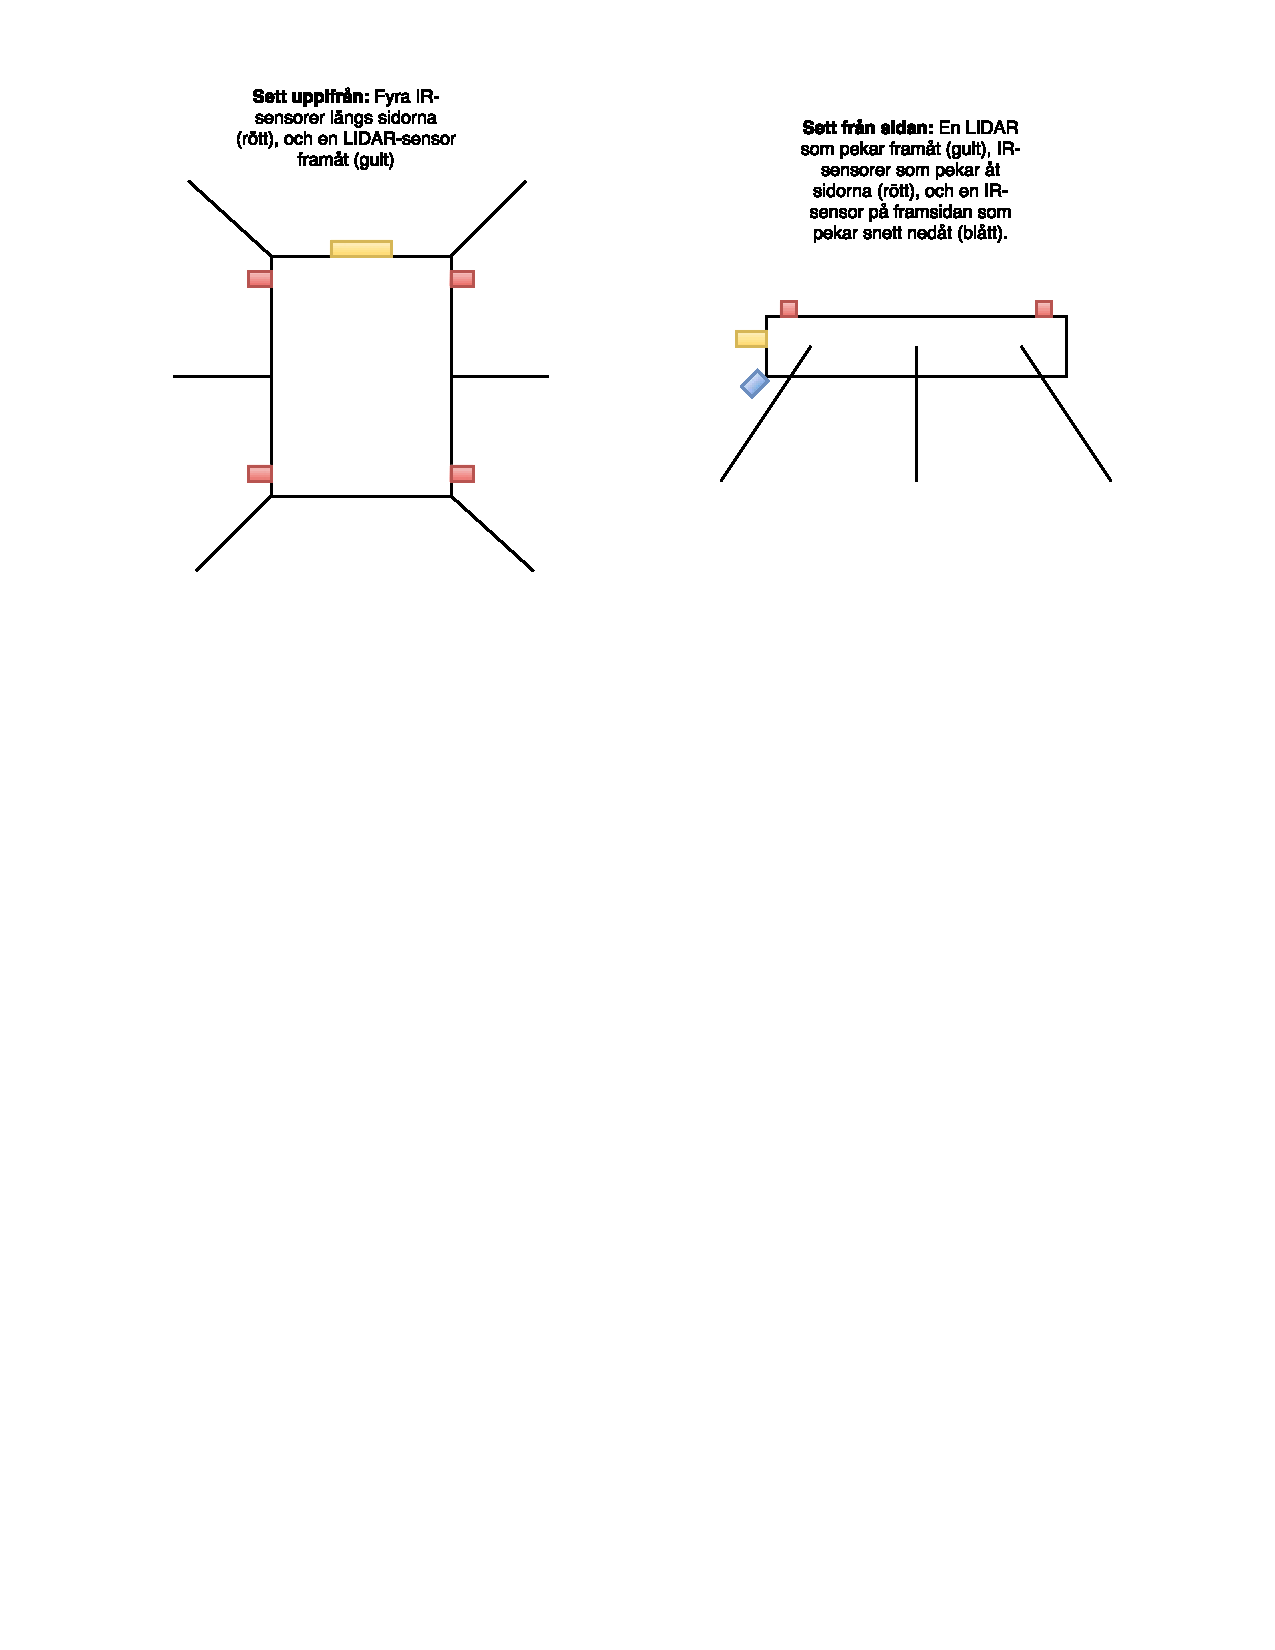
\includegraphics[width=17cm, trim=2cm 18cm 0cm 0cm]{images/sensor_mount.pdf}
        \caption{Montering av avståndssensorer\label{fig:sensor_mount}}
    \end{figure}

    \newpage
    \subsection{Krets}

    \begin{figure}[h]
        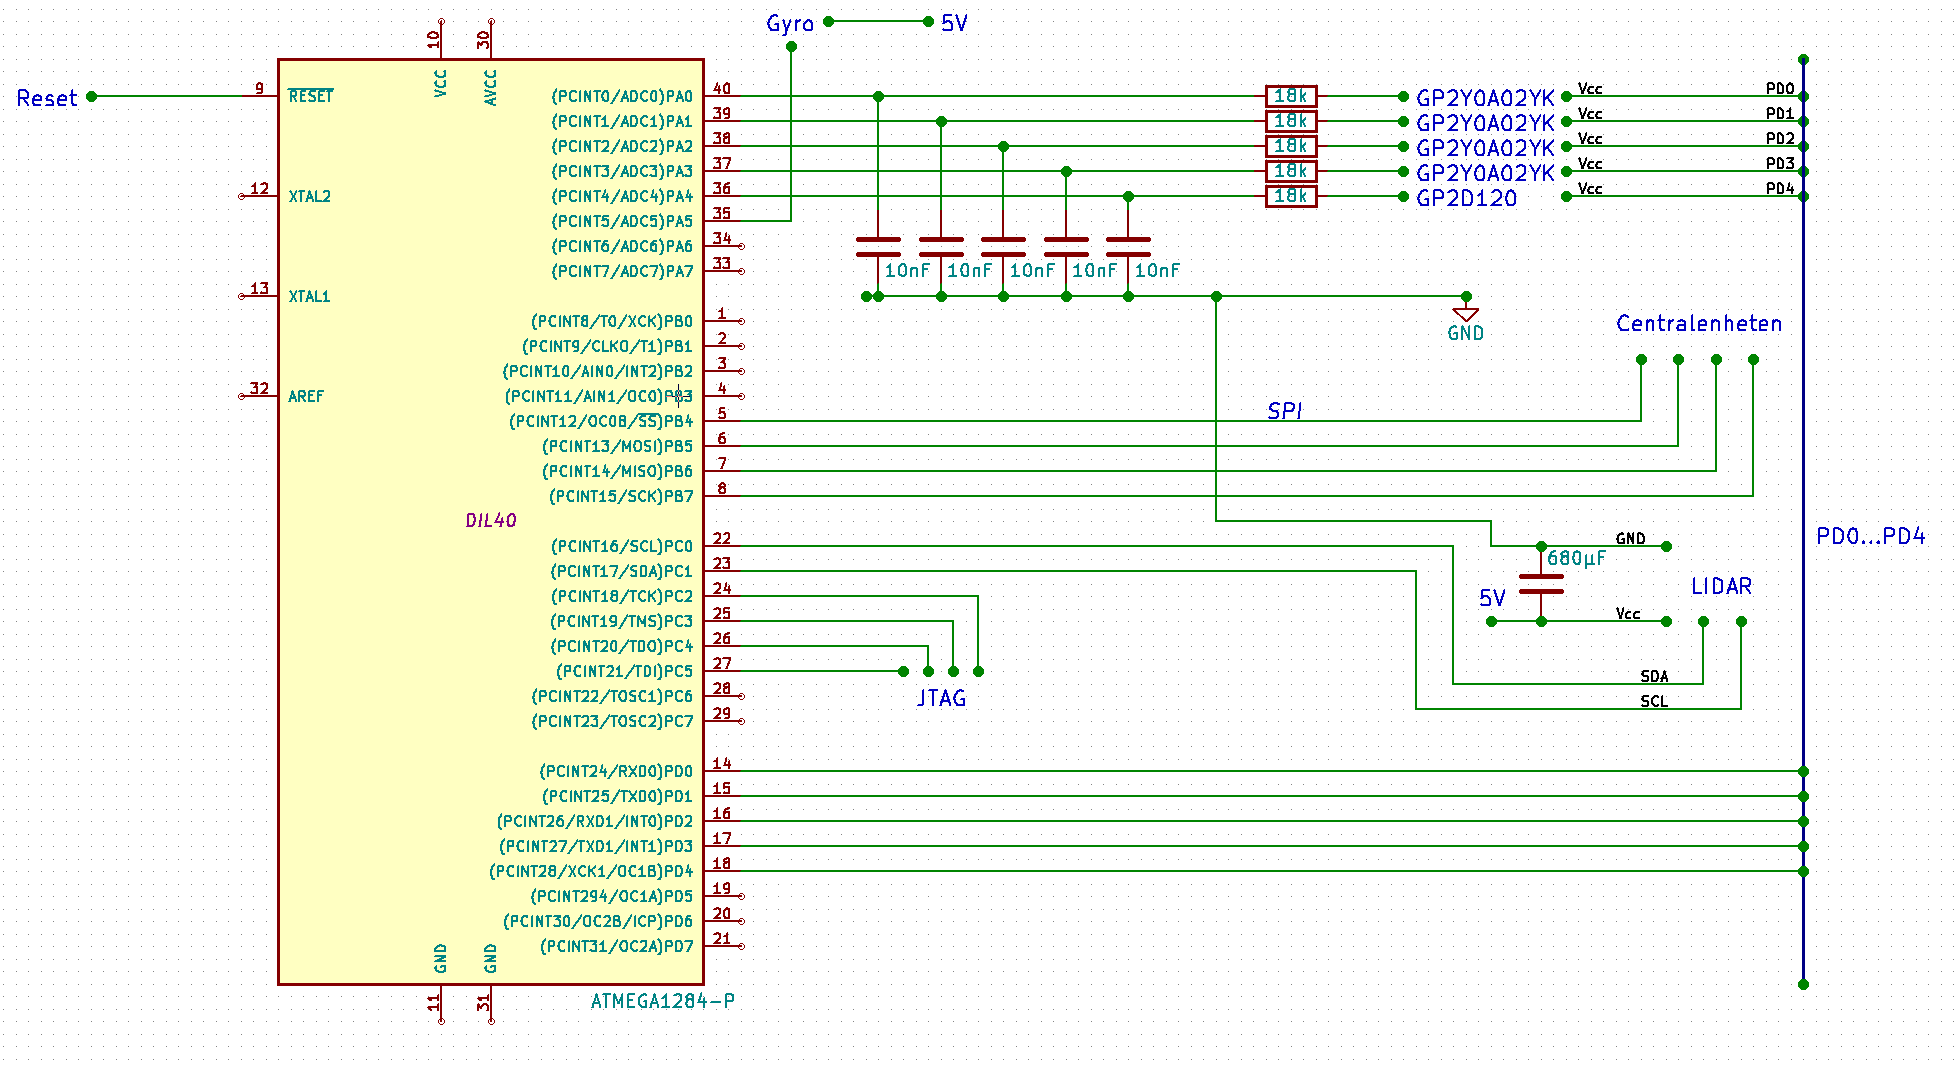
\includegraphics[width=15cm]{images/schematic_sensor.png}
        \caption{Kretschema över sensorenheten\label{fig:schem_sensor}}
    \end{figure}

    Ett antal lågpass-filter används för filtrering av brus från IR-sensorerna
    och utgörs av en kondenstator på 10nF och en 18kOhm-resistor för varje
    sensor. Filtret är kopplad mellan sensorerna och de analoga PA-ingångarna på
    processorn.

    LIDAR-sensorn är ansluten via PWM till ???VILKEN\_PORT??? på processorn.

    PC2 upp till PC5 används som anslutning till JTAG, för programmering av
    processorn, och PB4 upp till PB7 är anslutna via SPI till centralenheten.

    Figur \ref{fig:schem_sensor} visar ett kretschema över sensorenheten.

	
	%%%%%%%%%%%%%%%%%%%%%%%%%%%%%%%%%%%%%%%%%%%%%%%%%%%%%%%%%%%%%%%%%%%%%%%%%%%%%%%%%
	%						Grafiskt användargränssnitt
	%%%%%%%%%%%%%%%%%%%%%%%%%%%%%%%%%%%%%%%%%%%%%%%%%%%%%%%%%%%%%%%%%%%%%%%%%%%%%%%%%

    \newpage
	\section{Grafiskt användargränssnitt}
	På centralenheten körs en webbserver som tillhandahåller ett gränssnitt för
    användaren där man kan läsa sensordata eller kontrollera roboten i manuellt
    läge. Front-end-delen är skriven i Elm och back-end-delen i Elixir med hjälp
    av webbramverket Phoenix. På webbservern körs också RabbitMQ som används som
    en kommunikationsserver mellan centralenheten och webbservern/gui:t. Se
    \ref{gui:kommunikation} Kommunikation nedan.

	I det manuella läget styrs roboten med en joystick som är kopplad till
    användarens dator eller med knappar på gränssnittet. Figur
    \ref{fig:gui-overview} visar en illustration av det grafiska gränssnittet.
	
	\begin{figure}[h]
		\centering
		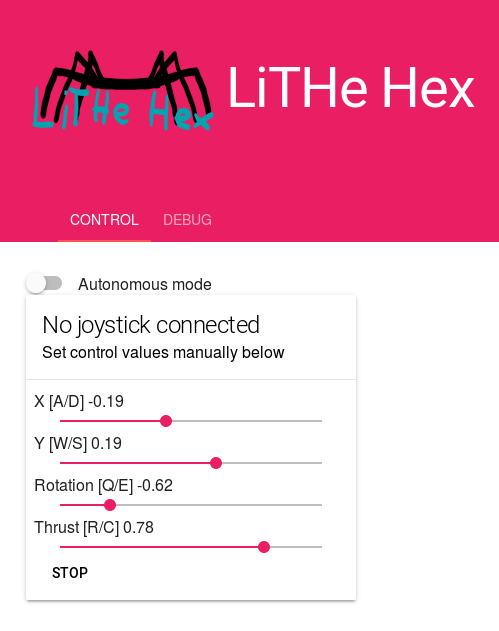
\includegraphics[width=0.5\linewidth]{images/gui-index.png}
		\caption{Det grafiska gränssnittet\label{fig:gui-overview}}
	\end{figure}

	\subsection{Webbserver}
	Webbservern är skriven i Elixir och använder webbramverket Phoenix. Kommunikationen mellan frontend och backend sker via en channel. En channel är en socket som tillåter kommunikation mellan en klient och en server. I channeln så skickas det från frontend till backend styrdata, d.v.s, joystickdata och om det autonoma läget ska köras eller inte. Från backend till frontend skickas debugdata som IR-sensorer, LIDAR samt vinklar.
	
	% Är det varje 0.3 sekund?
	Backend skickar styrdatan till RabbitMQ servern som centralenheten sedan
	läser av. Det skickas varje 0.3 sekund till RabbitMQ servern.

    \subsection{Styrning}
    Under styrning kan man välja om roboten ska köras autonomt eller i manuellt läge.
    För att ändra vilket läge roboten ska köras i finns en knapp som växlar dess läge.
    
    % TODO: Kan man verkligen styra med tangentbordet??
    \subsubsection{Manuell Styrning}
    Under styrning man man styra roboten med en joystick. Man kan även
    styra roboten med tangentbord eller knappar på skärmen. För att styra
    roboten finnas knappar som säger åt roboten att gå i en riktning,
    att vrida sig åt ett håll och att stanna.

	% TODO: Stämmer det med 10 gånger per sekund? Kan man ändra styrparamterarna till regleralgoritmen?
    \subsection{Debug}
	Under debug visas robotens olika inställningar samt sensordata vid
    tillfället. Sidan uppdateras 10 gånger per sekund och klienten får den
    uppdaterade data:n med hjälp av JSON. Det finns också flera grafer
    som beskriver några av de olika sensorernas data. Man kan också ändra
    styrparametrarna till regleralgoritmen.

	\label{gui:kommunikation}
    \subsection{Kommunikation}

	\begin{longtable}[c]{l l l }
        \textbf{Data} & \textbf{Nyckel} & \textbf{Typ} \\ \midrule
        IR-sensor ned & "ir\_down" & float \\
        IR-sensor fram vänster & "ir\_fl" & float \\
        IR-sensor fram höger & "ir\_fr" & float \\
        IR-sensor bak vänster & "ir\_bl" & float \\
        IR-sensor bak höger & "ir\_br" & float \\
        LIDAR & "lidar" & float \\
        Vinkel till vänster vägg & "angle\_l" & float \\
        Vinkel till höger vägg & "angle\_r" & float \\
        Genomsnittlig vinkel & "angle\_avg" & float \\
        Självgående läge & "auto" & bool \\
        Debugsträng & "debug" & string \\

		\caption{Format på JSON-strängen från
        centralenheten\label{table:guimessagesfromcentral}}
	\end{longtable}

	\begin{longtable}[c]{l l l }
        \textbf{Data} & \textbf{Nyckel} & \textbf{Typ} \\ \midrule
        X-hastighet & "x" & float \\
        Y-hastighet & "y" & float \\
        Rotation & "rotation" & float \\
        Thrust & "thrust" & float \\
        Självgående läge & "auto" & bool \\

		\caption{Format på JSON-strängen till
        centralenheten\label{table:guimessagestocentral}}
	\end{longtable}
    

	%%%%%%%%%%%%%%%%%%%%%%%%%%%%%%%%%%%%%%%%%%%%%%%%%%%%%%%%%%%%%%%%%%%%%%%%%%%%%%%%%
	%						Simuleringar
	%%%%%%%%%%%%%%%%%%%%%%%%%%%%%%%%%%%%%%%%%%%%%%%%%%%%%%%%%%%%%%%%%%%%%%%%%%%%%%%%%
    \newpage
	\section{Simuleringar}
	För att underlätta utvecklingen av vissa delar av projektet har vi att
    skrivit kod för att simulera dessa delar. Simuleringarna kör samma kod som
    ska köras på roboten men visualisera resultatet utan resten av roboten. De
    delar där simulering är mest aktuellt är inverterad kinematik,
    korridorföljning och gångstil.

	\subsection{Simulering för inverterad kinematik}
	Simuleringen går till genom att implementera algoritmen för 2D som beskrivs
    i avsnitt \ref{sub:inverterad-kinematik}. Simuleringen ritas sedan ut i
    webbläsaren för att visualisera den inverterade kinematiken. Den här
    simuleringen är skriven i Elm.
	
	\subsection{Simulering för korridorföljning}
	Simulering för korridorföljning kan testa olika regleralgoritmer utan att
    behöva testa dem på en gående robot. Simuleringen ritar ut en korridor och
    en robot som går framåt. Simulatorn skickar ut sensorvärden till en fil,
    regleralgoritmen läser in sensorvärden och tar sedan beslut. Roboten i
    simulatorn använder 2 IR-sensorer på varje sida som pekar rakt ut från
    roboten, det går att välja var på roboten som sensorerna ska sitta. Beslutet
    av regleralgoritmen skrivs till en fil som simulatorn läser in och styr
    roboten efter det. Det finns möjlighet att lägga till en störningsfunktion
    som till exempel kan vara att roboten alltid går med en liten rotation.
	
	\subsection{Simulering för gångstil}
	Simulatorn för gångstil fungerar på samma sätt som
    korridorföljningssimulatorn. Motorikenhetens kod skriver informationen som
    på roboten skulle skickas till servona till en fil som simulatorn läser.
    Simulatorn visualiserar resultatet av kommandona och skriver data som
    servona skulle svara med till en annan fil som motorikkoden kan läsa.

\end{document}
